\documentclass[a4paper,12pt]{article}

\usepackage{balance}
\usepackage{graphicx}
\usepackage{booktabs}
\usepackage{relsize}
\usepackage{pgfplots}
\usepackage{tabularx}
\usepackage{gensymb}
\usepackage{caption}
\usepackage{listings}
\usepackage{babel}
\usepackage{siunitx}
\usepackage{url}
\usepackage{subcaption}
\usepackage{comment}
\usepackage{tikz}


\usepackage[utf8]{inputenc}
\usepackage{amsmath}
\usepackage{hyperref}

\title{IoT-NDN: Ein Überblick über eine IoT-Architektur mittels Named Data Networking}
\author{Leonard Boetefuer}
\date{\today}

\begin{document}

\maketitle

\begin{abstract}
als Leztes
\end{abstract}

\section{Einleitung}
als vorleztes
\
XYZTEST2
\section{Hauptmerkmale von IoT-NDN}
\begin{itemize}
\item Related Work
\item Analysis of IoT and NDN\\
    A$)$ Challenges of IoT\\
    \begin{enumerate}
        \item The connection of IoT devices
        \item Technology Standards
        \item Mobility
        \item Complexity of Integration Issues
    \end{enumerate}
    B$)$ NDN for IoT\\
    \begin{enumerate}
        \item NDN Packet Lenght
        \item Caching in IoT/NDN
        \item Data Aggregation in Wireless Networks:
        \item Naming Problems in Wirless Networks
        \item Routing Scalability in NDN:
    \end{enumerate}
\item Architecture of IoT-NDN System\\
    graphics and stuff\\
    A$)$ Naming\\
    B$)$ Management and Control Plane\\
    \begin{itemize}
        \item Aggregation
        \item Controlled Flooding
        \item Name-Centric Service
    \end{itemize}
    C$)$ Data PLane\\
    \begin{itemize}
        \item Strategy-In-Network Caching
        \item Strategy-Forwarding
    \end{itemize}
    
\end{itemize}

related Work

short introduction\\

A$)$ Challenges 1-5\\





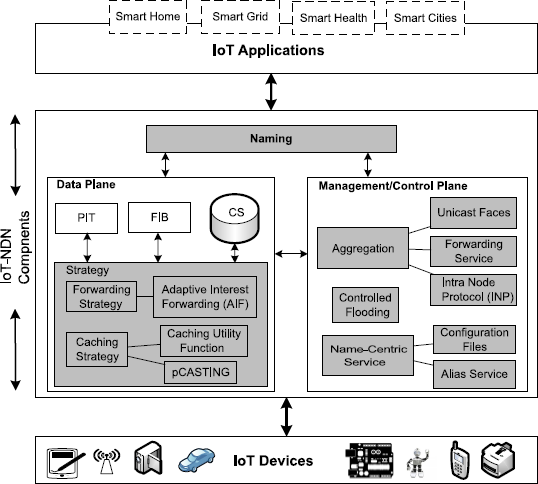
\includegraphics[width=0.5\textwidth]{IoT-NDN_System_architecture_and_its_components.png}\\
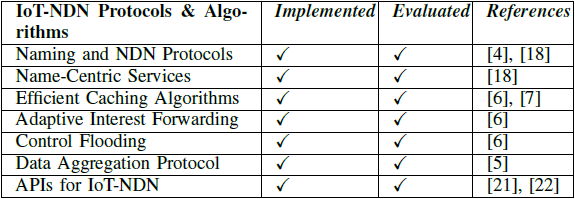
\includegraphics[width=0.5\textwidth]{IMPLEMENTED_AND_TESTED_PROTOCOLS_AND_ALGORITHMS_IN_IOT-NDN.png}\\
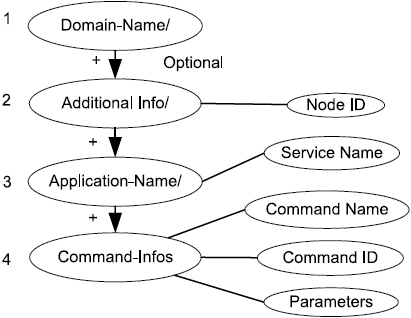
\includegraphics[width=0.5\textwidth]{Name_Structure_of_the_suggested_Approach.png}\\
\section{Fazit}
XYZ
\section{References}
XYZ
\end{document}